\documentclass[leqno]{article}
\usepackage[utf8]{inputenc}
\usepackage{enumitem}
\usepackage{tikz}
\usepackage[parfill]{parskip} % Don't start new paragraph with tab.
\usepackage{amsmath} % For \tag and \eqref

\title{Computationele logica}
\author{
    \small Kamans, Jim\\
    \texttt{10302905}
    \and
    \small Hendrikse, Mila\\
    \texttt{00000000}
    \and
    \small Roosingh, Sander\\
    \texttt{11983957}
    \and
    \small Schenk, Stefan\\
    \texttt{11881798}
}
\date{November 2017}

\begin{document}

\maketitle


%%%%%%%%%%%%%%%%
%% Exercise 1 %%
%%%%%%%%%%%%%%%%
\section{Exercise 1}

\begin{enumerate}

    \item The sentence $\theta$ encoding all information: \\
    $\theta$ = $K_a r_b \wedge \neg (K_a r_a \vee K_a w_a)
            \wedge K_b r_a \wedge \neg (K_b r_b \vee K_b w_b)
            \wedge K_q r_a \wedge K_q r_b$ \\

    \item A representation of the situation model \textbf{M}: \\
    $\mathcal{A}$ = \{a, b, q\} the agents Alice, Bob, and the Queen \\
    $\Phi$ = $\{r_a, w_a, r_b, w_b\}$ the colors of the hats for a and b \\

    \begin{center}
    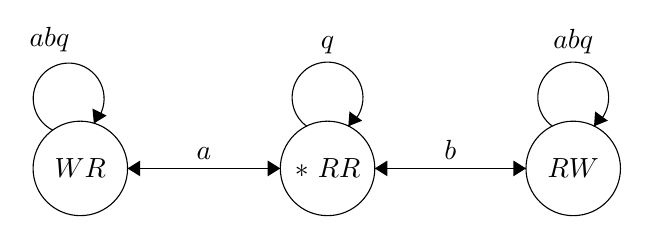
\begin{tikzpicture}[scale=0.2]
    \tikzstyle{every node}+=[inner sep=0pt]
    \draw [black] (38.4,-13.7) circle (3);
    \draw (38.4,-13.7) node {$*\mbox{ }RR$};
    \draw [black] (54,-13.7) circle (3);
    \draw (54,-13.7) node {$RW$};
    \draw [black] (22.7,-13.7) circle (3);
    \draw (22.7,-13.7) node {$WR$};
    \draw [black] (41.4,-13.7) -- (51,-13.7);
    \fill [black] (51,-13.7) -- (50.2,-13.2) -- (50.2,-14.2);
    \draw (46.2,-13.2) node [above] {$b$};
    \draw [black] (51,-13.7) -- (41.4,-13.7);
    \fill [black] (41.4,-13.7) -- (42.2,-14.2) -- (42.2,-13.2);
    \draw [black] (35.4,-13.7) -- (25.7,-13.7);
    \fill [black] (25.7,-13.7) -- (26.5,-14.2) -- (26.5,-13.2);
    \draw (30.55,-13.2) node [above] {$a$};
    \draw [black] (25.7,-13.7) -- (35.4,-13.7);
    \fill [black] (35.4,-13.7) -- (34.6,-13.2) -- (34.6,-14.2);
    \draw [black] (37.077,-11.02) arc (234:-54:2.25);
    \draw (38.4,-6.45) node [above] {$q$};
    \fill [black] (39.72,-11.02) -- (40.6,-10.67) -- (39.79,-10.08);
    \draw [black] (52.677,-11.02) arc (234:-54:2.25);
    \draw (54,-6.45) node [above] {$abq$};
    \fill [black] (55.32,-11.02) -- (56.2,-10.67) -- (55.39,-10.08);
    \draw [black] (20.955,-11.274) arc (243.46232:-44.53768:2.25);
    \draw (20.74,-6.36) node [above] {$abq$};
    \fill [black] (23.56,-10.84) -- (24.37,-10.35) -- (23.47,-9.9);
    \end{tikzpicture}
    \end{center}

    This is an epistemic model: NO, the model is not reflexive. \\

    \item Seperately a and b look in their mirrors and see their red hats, represented in the event model $\Sigma$ with four actions: \\

    This is an epistemic model: YES / NO \\
    This is a doxasic model: YES / NO \\

    \item The update product of the two models \textbf{M} $\bigotimes$ $\Sigma$ : \\

    This is an epistemic model: YES / NO \\
    This is a doxasic model: YES / NO \\

\end{enumerate}


%%%%%%%%%%%%%%%%
%% Exercise 2 %%
%%%%%%%%%%%%%%%%
\section{Exercise 2}

\begin{enumerate}

    \item There are ? possible worlds.
    \item
    \item
    \item
    \item

\end{enumerate}


%%%%%%%%%%%%%%%%
%% Exercise 3 %%
%%%%%%%%%%%%%%%%
\section{Exercise 2}

\begin{enumerate}

    \item
    \item
    \item
    \item
    \item
    \item
    \item
    \item
    \item

\end{enumerate}


\end{document}


